\section{Écriture du code}

Cette partie explique toutes les fonctions que nous avons écrites, complétées ou rajoutées dans le fichier \\ \texttt{demo\_control\_polycopie2023.py}.

\subsection{Calcul de l'énergie}

\subsubsection{Description de l'algorithme}

Tout d'abord, la première fonction que nous avons écrite est celle permettant de calculer l'énergie $J(\chi) := \int_\Omega |p_\chi|^2dx$. Cette fonction est appelée \texttt{your\_compute\_objective\_function} dans le code. Afin d'approcher l'intégrale permettant de calculer l'énergie, nous utilisons l'algorithme suivant:

\begin{itemize}
    \item Prendre un point du maillage qui possède un voisin à droite et en bas;
    \item Vérifier si le carré formé par le point initial, son voisin en bas, son voisin à droite et son voisin en bas à droite est dans l'intérieur du domaine;
    \item Si c'est le cas, calculer la moyenne de la valeur absolue au carré des points du carré;
    \item Multiplier cette moyenne par l'aire du carré, cela nous donne une approximation de l'énergie dans le carré;
    \item Faire ceci pour tous les points qui ont un voisin à droite et en bas.
\end{itemize}

Cette formule de l'approximation de l'aire de la courbe d'une fonction à deux variables vient de \cite{4} et s'écrit, pour une fonction $f$ définie sur les coins du rectangle $[a, b]\times[c, d]$ et qui satisfait certaines conditions:
$$\displaystyle \int_a^b \int_c^d f(x,y)dy dx = [f(a,c) + f(a, d) + f(b, c) + f(b, d)]\frac{(b-a)(d-c)}{4} + E(f)$$ avec $E(f)$ l'erreur qui dépend des conditions sur $f$.\\ \\
De plus, pour vérifier que le carré considéré est bien dans le domaine et non pas à l'extérieur, il faut qu'au minimum un des points du carré soit à l'intérieur. Cette condition permet de bien prendre en compte l'énergie qui entre la frontière et l'intérieur dans la discrétisation.

\subsubsection{Implémentation en Python}

\begin{Python}
def your_compute_objective_function(domain_omega, u, spacestep):
    energy = 0.0
    for i in range(0, M-1):
        for j in range(0, N-1):
            if domain_omega[i, j] == _env.NODE_INTERIOR or domain_omega[i+1, j] == _env.NODE_INTERIOR or domain_omega[i, j+1] == _env.NODE_INTERIOR or domain_omega[i+1, j+1] == _env.NODE_INTERIOR:
                energy += (numpy.abs(u[i, j])**2 + numpy.abs(u[i+1, j])**2 + numpy.abs(u[i, j+1])**2 + numpy.abs(u[i+1, j+1])**2)*spacestep*spacestep/4
    return energy
\end{Python}

\subsection{Algorithme du gradient}

\subsubsection{Présentation théorique}

Afin d'optimiser de trouver la configuration optimale pour laquelle l'énergie est la plus basse dans notre domaine, il faut que nous minimisions l'énergie. Vu que cette dernière dépend de plusieurs variables, nous devons employée une méthode valable pour plusieurs variables. La méthode employée a été celle de la méthode de descente de gradient. Cela consiste à minimiser une fonction réelle différentiable dans un espace euclidien. \\ \\
Dans notre problème la fonction à minimiser est $ \chi \mapsto J(\chi)$. $J$ est bien différentiable au sens de Fréchet avec $J'(\chi) : L^{\infty}(\Gamma_{abs}) \to L^1(\Gamma_{abs})$ telle que:
$$J(\chi + \chi_0) = J(\chi) + \langle J'(\chi), \chi_0 \rangle + o(\chi_0)\,, \lim_{||\chi_0||_{\infty} \to 0} \displaystyle \frac{|o(\chi_0)|}{||\chi_0||_{\infty}} = 0.$$
L'algorithme du gradient va nous amener à considérer la suite $(\chi^{(n)})_{n \ge 0}$ définie par la relation:
$$ \chi^{(k+1)} = \mathcal{P}_{\ell_k}\big[\chi^{(k)} - \mu_k J'(\chi^{(k)})\big]$$
où $\mathcal{P}_{\ell_k}$ est un projecteur visant à restreindre $\chi^{(k)} - \mu_k J'(\chi^{(k)})$ dans $[0, 1]$ et garantir $\beta = \displaystyle \int_{\Gamma_{abs}}\chi^{(k+1)}  dS$, et où $\mu_k > 0$ est un paramètre, recalculé à chaque étape, défini comme le taux d'apprentissage. Nous parlerons de $\mathcal{P}_{\ell_k}$ juste après.\\ \\
Si à l'itération $k+1$ nous n'arrivons pas à diminuer l'énergie par rapport à l'itération $k$, nous divisions par $2$ le taux d'apprentissage $\mu_k$ et nous recalculons $\chi^{(k+1)}$. Cependant si l'énergie est bel et bien diminuée, alors on augmente $\mu_k$. Le pseudo code de l'algorithme est en présent en Figure 2. 

\begin{figure}[H]
    \centering
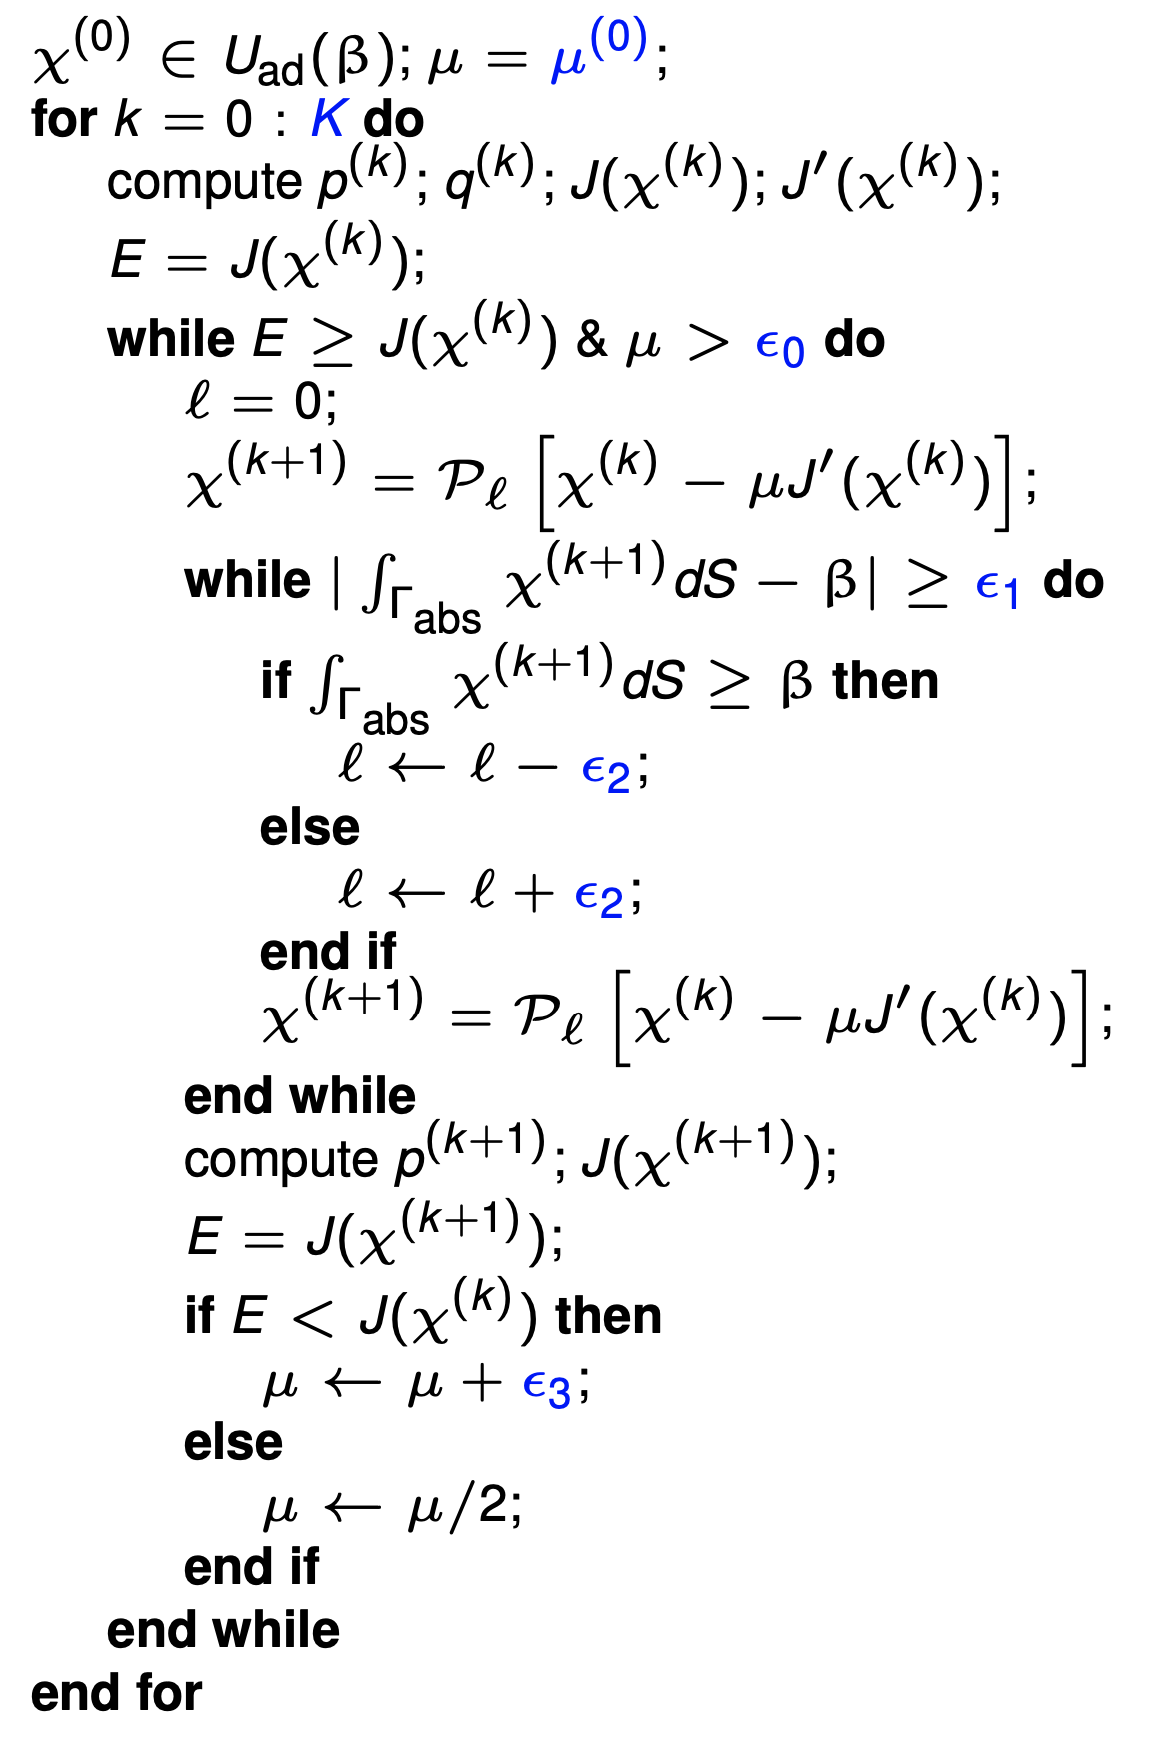
\includegraphics[width=0.3\linewidth]{rapport/numerique/assets/pseudo_code.png}
    \caption{Pseudo-code de l'algorithme du gradient appliqué à notre problème}
    \label{fig:enter-label}
\end{figure}

De ce fait, la suite $(J(\chi^{(n}))_{n \ge 0}$ va être amenée à converger théoriquement vers un minimum de $J$ car $\forall k > 0,$:
\begin{align*}
    J(\chi^{(k+1)}) - J(\chi^{(k)}) &= J(\chi^{(k)}) + \langle J'(\chi^{(k)}), -\mu_k J'(\chi^{(k)}) \rangle - J(\chi^{(k)}) + o(\mu_k J'(\chi^{(k)}))\\ 
    &= -\mu_k ||J'(\chi^{(k)})||^2 + o(\mu_k J'(\chi^{(k)})).
\end{align*}

et, avec la définition de la dérivée de Fréchet, 

\begin{equation*}
    \lim_{||\mu_k J'(\chi^{(k)})||_{\infty} \to 0} \displaystyle \frac{|o(\mu_k J'(\chi^{(k)}))|}{||\mu_k J'(\chi^{(k)})||_{\infty}} = \lim_{\mu_k \to 0} \displaystyle \frac{|o(\mu_k J'(\chi^{(k)}))|}{||\mu_k J'(\chi^{(k)})||_{\infty}} = \lim_{\mu_k \to 0} \displaystyle \frac{|o(\mu_k J'(\chi^{(k)}))|}{|\mu_k||| J'(\chi^{(k)})||_{\infty}} = \lim_{\mu_k \to 0} \displaystyle \frac{|o(\mu_k J'(\chi^{(k)}))|}{|\mu_k||| J'(\chi^{(k)})||^2_{\infty}} = 0.
\end{equation*}

D'après le polycopié de ST \cite{3}, nous avons $J'(\chi) = - \text{Re}(\alpha p_\chi q_\chi)$ où $q_\chi$ est la solution du système adjoint de $(P_\chi)$.

\begin{equation}
    \tag{$P'_\chi$}
    \begin{cases}
    \Delta q + k^2 q = -2\bar{p_\chi} \text{ dans } \Omega \\
    q = 0 \text{ sur } \Gamma_{in} \\
    \displaystyle \frac{\partial q}{\partial n} = 0 \text{ sur } \Gamma \\[5pt]
    \displaystyle \frac{\partial q}{\partial n} + \alpha \chi q = 0 \text{ sur } \Gamma_{abs}
    \end{cases}
\end{equation}

\newpage

\subsubsection{Implémentation en Python}

\begin{Python}
def your_optimization_procedure(domain_omega, spacestep, omega, f, f_dir, f_neu, f_rob, beta_pde, alpha_pde, alpha_dir, beta_neu, beta_rob, alpha_rob, Alpha, mu, chi, V_obj):
    g_dir = numpy.zeros(f_dir.shape)
    g_neu = numpy.zeros(f_neu.shape)
    g_rob = numpy.zeros(f_rob.shape)
    k = 0
    (M, N) = numpy.shape(domain_omega)
    numb_iter = 1000
    energy = numpy.zeros((numb_iter+1, 1), dtype=numpy.float64)
    
    while k < numb_iter and mu > 10**(-5):
        print('---- iteration number = ', k)
        
        # print('1. computing solution of Helmholtz problem, i.e., u')
        u = processing.solve_helmholtz(domain_omega, spacestep, omega, f, f_dir, f_neu, f_rob, beta_pde, alpha_pde, alpha_dir, beta_neu, beta_rob, alpha_rob)
        
        # print('2. computing solution of adjoint problem, i.e., p')
        q = processing.solve_helmholtz(domain_omega, spacestep, omega, -2*numpy.conjugate(u), g_dir, f_neu, f_rob, beta_pde, alpha_pde, alpha_dir, beta_neu, beta_rob, alpha_rob)
        
        # print('3. computing objective function, i.e., energy')
        energy[k] = your_compute_objective_function(domain_omega, u, spacestep)
        ene = energy[k]
        
        # print('4. computing parametric gradient')
        grad = - numpy.real(Alpha*u*q)
        number_steps = 0
        
        while ene >= energy[k] and mu > 10**(-5):
            ene_list = numpy.array([])
            mu_list = numpy.array([])
            
            # print('    a. computing gradient descent')
            new_chi = compute_gradient_descent(chi, grad, domain_omega, mu)
            
            # print('    b. computing projected gradient')
            new_chi = compute_projected(new_chi, domain_omega, V_obj)
            
            # print('    c. computing solution of Helmholtz problem, i.e., u')
            new_alpha_rob = Alpha*new_chi
            new_u = processing.solve_helmholtz(domain_omega, spacestep, omega, f, f_dir, f_neu, f_rob, beta_pde, alpha_pde, alpha_dir, beta_neu, beta_rob, new_alpha_rob)
            
            # print('    d. computing objective function, i.e., energy (E)')
            ene = your_compute_objective_function(domain_omega, new_u, spacestep)
            
            mu_list = numpy.append(mu_list, mu)
            ene_list = numpy.append(ene_list, ene)
\end{Python}
\begin{Python}    
            bool_a = ene < energy[k]
            if bool_a:
                # The step is increased if the energy decreased
                mu = mu * 1.1
            else:
                # The step is decreased is the energy increased
                mu = mu / 2
            number_steps += 1
            print("mu=" + str(mu), "ene=" + str(ene), "grad=" + str(numpy.linalg.norm(grad, numpy.infty)), "old ene=" + str(your_compute_objective_function(domain_omega, u, spacestep)))
        mu = mu_list[numpy.where(numpy.min(ene_list) == ene_list)][0]
        chi = compute_gradient_descent(chi, grad, domain_omega, mu)
        chi = compute_projected(chi, domain_omega, V_obj)
        alpha_rob = Alpha*chi
        k += 1
    energy[k] = ene
    # print('end. computing solution of Helmholtz problem, i.e., u')
    return chi, energy, u, grad
\end{Python}

\subsection{Projection de $\chi$}

Afin de restreindre $\chi^{(k+1)}$ dans $[0, 1]$ et garantir que la quantité de matériaux $\beta$ reste constante au cours des itérations, nous devons utiliser un projeteur.

\subsubsection{Calcul de $\beta$}

Premièrement, vu que $\chi$ est une fonction caractéristique, pour calculer cette quantité de matériaux numériquement,  il faut sommer toutes les valeurs de $\chi$.\\ \\
Dans le code nous travaillerons régulièrement avec la proportion de matériaux définie par $$V = \displaystyle \frac{\displaystyle \int_{\Gamma_{abs}}\chi dS}{\displaystyle \int_{\Gamma_{abs}}dS}.$$

\subsubsection{Implémentation en Python du calcul de $\beta$}

\begin{Python}
def compute_projected(chi, domain, V_obj):
    (M, N) = numpy.shape(domain)
    S = 0
    for i in range(M):
        for j in range(N):
            if domain[i, j] == _env.NODE_ROBIN:
                S = S + 1
    B = chi.copy()
    l = 0
    chi = preprocessing.set2zero(chi, domain)

    V = numpy.sum(numpy.sum(chi)) / S
\end{Python}

\subsubsection{Calcul du projecteur}

Le projecteur utilisé est $\mathcal{P}_{\ell}(\chi) = \max(0, \min(\chi + \ell, 1))$ avec $\ell$ fixé de manière à garantir $\displaystyle \int_{\Gamma_{abs}}\chi^{(k)} = \beta$. En remarquant que la fonction $\ell \mapsto \displaystyle \int_{\Gamma_{abs}}\max(0, \min(\chi + \ell, 1))dS$ est croissante, il est possible de faire une dichotomie de manière à trouver le $\ell$ correspondant à cette condition. Les bornes utilisées pour $\ell$ sont $-\max(\chi)$ et 1. Vu que,
$$\displaystyle \int_{\Gamma_{abs}}\max(0, \min(\chi - \max(\chi), 1))dS = 0 \text{ et } \displaystyle \int_{\Gamma_{abs}}\max(0, \min(\chi + 1, 1))dS = \displaystyle \int_{\Gamma_{abs}}dS,$$
cela garantit que la dichotomie va trouver un $\ell$ qui va faire converger $\displaystyle \int_{\Gamma_{abs}}\max(0, \min(\chi + \ell, 1))dS$ vers $\beta$ car $0 \le \beta \le \displaystyle \int_{\Gamma_{abs}}dS.$

\subsubsection{Implémentation en Python du projecteur (suite du code du calcul de $\beta$)}

\begin{Python}
    debut = -numpy.max(chi)
    fin = 1
    ecart = fin - debut
    # We use dichotomy to find a constant such that chi^{n+1}=max(0,min(chi^{n}+l,1)) is an element of the admissible space
    while ecart > 10**(-5):
        # calcul du milieu
        l = (debut + fin) / 2
        for i in range(M):
            for j in range(N):
                chi[i, j] = numpy.maximum(0, numpy.minimum(B[i, j] + l, 1))
        chi = preprocessing.set2zero(chi, domain)
        V = sum(sum(chi)) / S
        if V > V_obj:
            fin = l
        else:
            debut = l
        ecart = fin - debut
        # print('le volume est', V, 'le volume objectif est', V_obj)

    return chi
\end{Python}

\subsection{Problèmes rencontrés dans l'optimisation}

Quelques problèmes se sont produits avec cette première version du code.
\begin{itemize}
    \item Le programme d'optimisation s'arrêtait au bout de quelques itérations seulement à cause du critère $\mu \ge 10^{-5}$ pour rester dans la grande boucle. En effet, vu que l'algorithme n'arrive pas à trouver une valeur de $\mu_k$ pour diminuer l'énergie, le $\mu_k$ est divisé par $2$ jusqu'à être inférieur à $10^{-5}$ pour sortir de la petite boucle. Nous avons donc penser à enlever ce critère de la petite boucle et de la grande boucle, et nous l'avons remplacé par un nombre maximal d'itérations dans la petite boucle.
    \item De même, vu que le $\mu_k$ devient trop petit à cause du blocage dans la petite boucle, nous avons décidé de rajouter $10^{-3}$ à $\mu_k$ à chaque passage dans la grande boucle. Cela à une grande influence si la petite boucle s'est exécutée un trop grande nombre de fois, et ne change pratiquement rien si l'énergie a bien été diminuée au bout de quelques essais seulement.
    \item Nous avons observé que le code convergeait beaucoup plus vite et beaucoup mieux en mettant un signe "+" devant le calcul du gradient. De cette manière nous avons réalisé une bonne partie de nos tests avec ce signe "+" sans avoir plus d'explications scientifiques. Suite à cet ajout, nous avons remis le critère sur $\mu_k$ dans la petite boucle et enlevé le rajout de $10^{-3}$.
\end{itemize}

\subsection{Projection final}

\subsubsection{Explication théorique}

La dernière étape de l'algorithme est de projeter le $\chi$ optimal calculé par l'algorithme dans l'ensemble discret $\{0,1\}$ tout en conservant la quantité de matériaux $\beta$.\\ \\
Pour ce faire, nous adoptons une projection de la forme 
\begin{align*}
    \mathcal{P_\mathcal{\gamma}} 
    \colon& \mathcal{F}(\Gamma_{abs}, [0, 1]) \longrightarrow \mathcal{F}(\Gamma_{abs},\{0,1\}) \\
    &\chi \mapsto \mathbf{1}_{\chi > \gamma},
\end{align*}
où $\gamma$ est choisi de manière à avoir $\displaystyle \int_{\Gamma_{abs}} \mathcal{P_\mathcal{\gamma}} (\chi)dS = \beta$. \\ \\
Numériquement, fixer $\gamma$ revient à déterminer le nombre de points de la liste \texttt{chi} qui doivent être égaux à $1$. Nous souhaitons donc qu'il y ait exactement $\lfloor \beta \rfloor$ points dans la liste \texttt{chi} ayant la valeur $1$. (Nous utilisons la partie entière inférieure car il est préférable d'utiliser moins de matériaux que prévu plutôt que d'en utiliser trop.) Pour les sélectionner, nous choisissons simplement les $\lfloor \beta \rfloor$ points ayant les valeurs les plus élevées.

\subsubsection{Implémentation en Python}

\begin{Python}
def final_projected(chi, nb_pixels):
    # find the beta th largest value of chi
    chi_copy = chi.copy()
    chi_copy = chi_copy.reshape(-1)
    chi_copy.sort()
    chi_copy = chi_copy[::-1]
    threshold = chi_copy[nb_pixels-1]
    # set to zero all the values of chi that are smaller than the threshold
    chi[chi < threshold] = 0.
    # set to one all the values of chi that are greater than the threshold
    chi[chi >= threshold] = 1.
    return chi
\end{Python}